\section{Materials and Methods}
\label{sec:m&ms}

\subsection{Subjects}

Three hand amputees, patients of the INAIL Centro Protesi in Vigorso
di Budrio, Bologna, Italy, joined the experiment voluntarily after
having been carefully informed of the procedure they were about to undergo,
according to the INAIL patients care guidelines. All of them have lost
their limb traumatically and, at the time of the experiment, the status of
their muscle remnants was excellent.

Subject $1$ is male, 63 years old, trans-radial
one-third proximal, amputated in 1963; he is a
pioneer of myoelectric prostheses, having started using them in the
Sixties. The Subject $2$ is male, aged 56, trans-radial one-third
distal, amputated in 1972; he also started using myoelectric prostheses
very early, actually in 1974. Subject $3$ is male as well, aged 25,
trans-carpal, amputated in 2007; he was in the process of learning how
to use a standard myoelectric prosthesis at the time the experiment was
performed (summer 2008). Subject $1$ has about $9$cm left of his
forearm, Subject $2$ has some $20$cm, and Subject $3$ has the whole forearm
plus some of the carpus --- see Figure \ref{fig:stumps}.

\begin{figure*}[!ht] \centering
  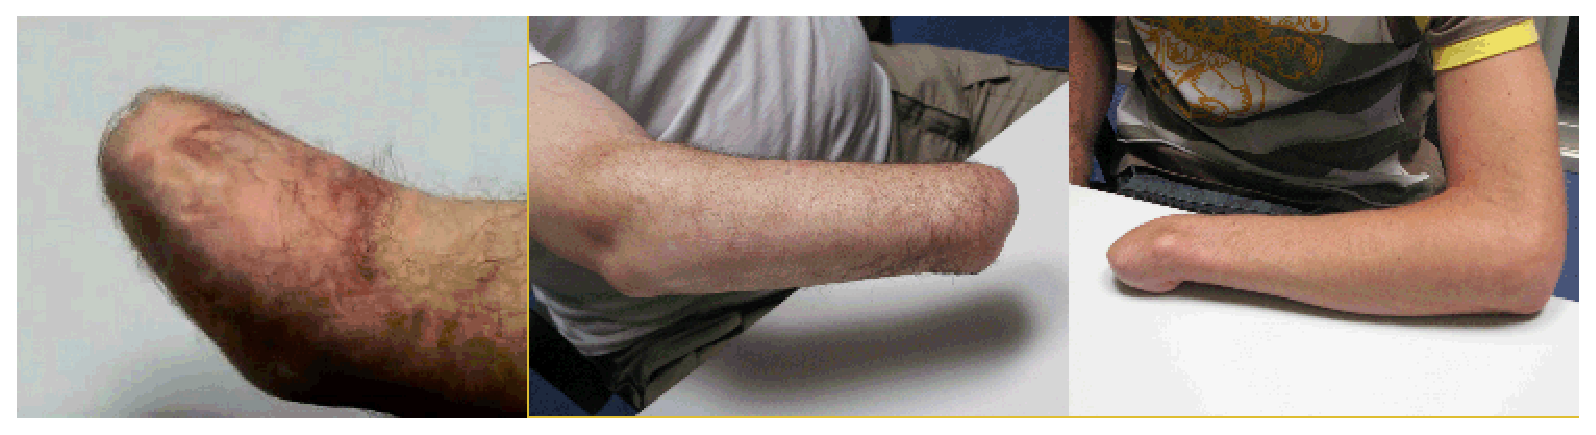
\includegraphics[width=\textwidth]{figs/stumps}
  \caption{the subjects' stumps. Subject $1$ (left) has a trans-radial
    one-third proximal amputation, with a stump about $9$cm long;
    Subject $2$ (center) is trans-radial one-third distal, stump about $20$cm
    long; Subject $3$ (right) is trans-carpal, retaining the full forearm.}
  \label{fig:stumps}
\end{figure*}

\subsection{Setup}

We used a FUTEK LMD500 Hand Gripper force sensor \cite{futek}, a strain-gauge
based sensor with guaranteed low non-linearity and hysteresis factors, which can easily
be gripped in various ways since it is light and small. The sensor returns a
voltage proportional to the force applied to its narrow face (Figure \ref{fig:setup}, left).
Also, $5$ standard commercial surface EMG electrodes were used, namely OttoBock
Myobock models \cite{myobock}, type 13E125=50 (Figure \ref{fig:setup}, center).
The electrodes are dry bi-differential with a frequency bandwidth ($-3$dB) of
$140$-$1500$Hz, adjustable amplification gain from $0$ to $50000$, CMMR of
$80$dB and a double T notch filter at $50$Hz (in the European version
that we used) for power supply interference rejection. After a few initial
experiments, we set the amplification at mid-range, which gave us an output voltage
exactly matching the input range of the acquisition card.
These electrodes are the state-of-the-art in commercially available myoprostheses,
since their output is deemed exceptionally good, highly correlated with the
force exerted by the muscle(s) whose activity the electrode is gathering.
All in all, six signals were monitored (one per each EMG electrode and one from the
force sensor), and sampled at a rate of $100$Hz via a standard USB acquisition card,
connected to an entry-level laptop.

\begin{figure*}[!ht] \centering
  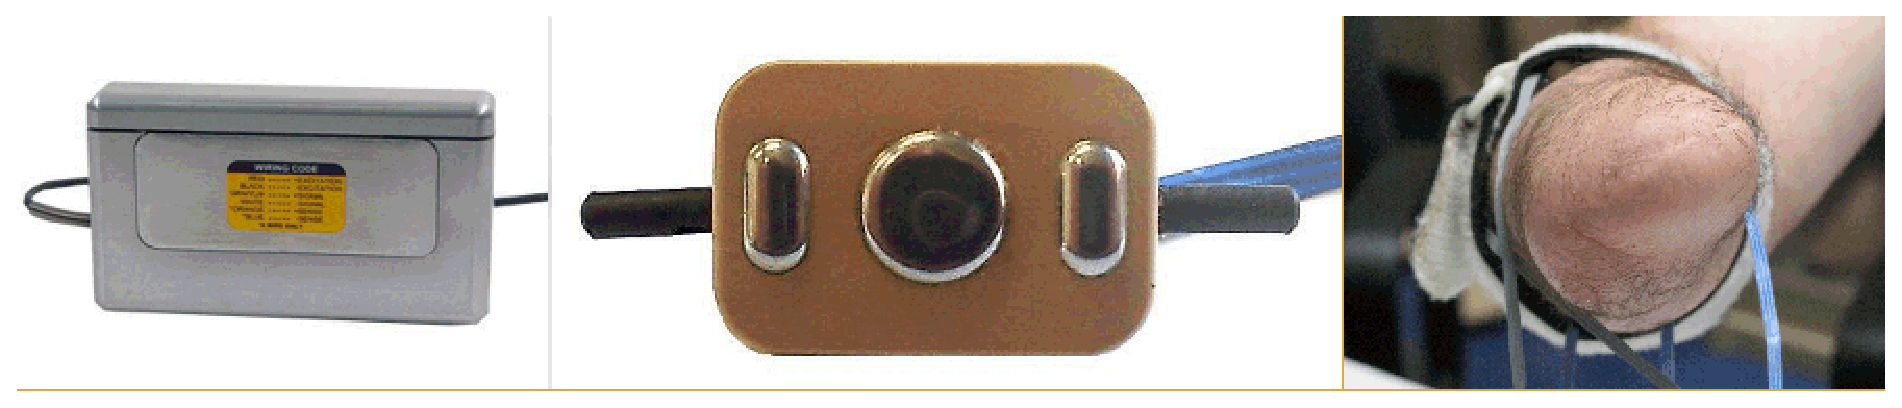
\includegraphics[width=\textwidth]{figs/setup}
  \caption{parts of the experimental setup. (left to right) the FUTEK LMD500
    Hand Gripper; an Otto Bock Myobock EMG electrode; placement of the electrodes
    on a subject's stump, parallel to the forearm axis, equally spaced, held in
    place by an elastic band --- the electrodes' wires are clearly seen.}
  \label{fig:setup}
\end{figure*}

The electrodes were placed around the stump just below the elbow, parallel
to the forearm axis, equally spaced and held in place by an elastic band
(Figure \ref{fig:setup}, right panel). This was done
in order to detect signals from all muscle remnants uniformly,
rather than try and associate electrodes to single muscles
as is the case in normal one-DOF myodevices. By the way, for Subject $1$
this was the only possibility, since his stump
would not allow the electrodes to be positioned anywhere else --- this problem
of ``cluttered'' electrodes on a subject's stump actually also appears in
\cite{sebelius}.

\subsection{Experimental procedure}

\subsubsection{Grasping postures}

The subjects were asked to perform with their phantom hand several
different grasp postures, chosen according to suggestions by the
INAIL Centro Protesi personnel and patients, and loosely based upon
Cutkosky's taxonomy \cite{cutkosky}:

\begin{enumerate}

  \item the baseline \emph{rest condition} (\re);

  \item the act of \emph{pointing the index finger} (\po), used when pressing buttons;

	\item a \emph{power grasp} (\pw) in which the whole hand wraps around an object,
		used, e.g., when holding a heavy cylindrical object such as a hammer;
		
	\item a \emph{precision pinch grip} (\pi) with thumb and index finger closing on
	 	an object, usually for lifting small objects such as a pen or an egg;
	
	\item a \emph{precision tripodal grip} (\tr) similar to \pi, but using the
		middle finger too, used for spherical objects;
		
	\item the act of \emph{stretching one's hand} (\hs), used when an amputee is trying
		to put his hand inside a pocket. 

\end{enumerate}
	
Each posture was performed repeatedly by each subject a free number of times,
ranging from $10$ to about $25$ (except the rest condition, obviously, which consisted
of a few seconds of no-activity recording), with speeds ranging from $5$Hz to
"slow motion" (about $20$ seconds to complete a grasp, using various degrees of
force). The postures were performed in the order described
above, with a few seconds of rest inbetween. The
experimenter would at times suggest the subject to go faster or slower, to press
harder or softer, and at times the subject would be free to do whatever he wanted.
We will call this sequence a \emph{cycle}.

\subsubsection{Training modalities}

Since we employ a supervised learning strategy, a way of knowing what the subject is
doing is required in the training phase. In particular, each sample must be associated
to a label, denoting the current grasp posture, and to a force value.

Labels, one for each required posture (\re,\po,\pw,\pi,\tr,\hs),
were attached to each sample simply according to the
type of grasp required from the subject during a particular phase of the current
cycle; for example, samples gathered while asking the subject to perform a power grasp
would be labled with \po, and so on.

\begin{figure*}[!ht] \centering
  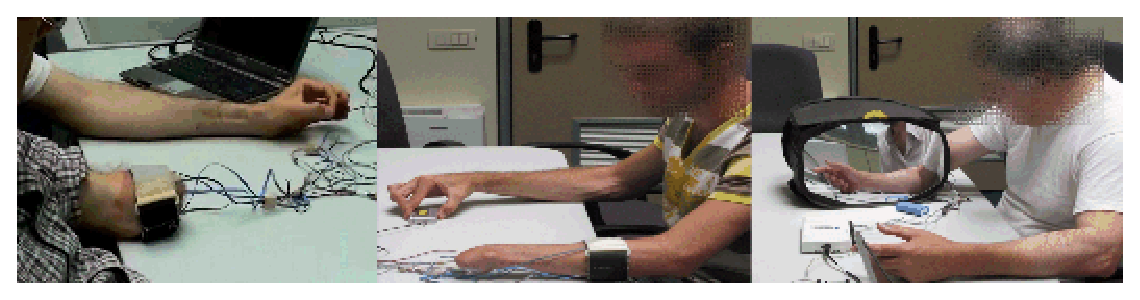
\includegraphics[width=\textwidth]{figs/modalities}
  \caption{the three training modalities. (left to right) Subject $1$
    imitating a pinch grip; Subject $3$ bilaterally performing a pinch
    grip; Subject $2$ assuming the pointing index posture while
    looking in the mirror-box.}
  \label{fig:modalities}
\end{figure*}

Force values, on the other hand, were collected according to three
\emph{modalities} (see Figure \ref{fig:modalities}):

\begin{enumerate}

  \item \emph{teacher imitation.} A healthy subject (the teacher)
    would place his arm besides the subject's stump and ask him
    to imitate the teacher's postures with his phantom limb. The
    subject was asked to grasp with maximum strength,
    while the teacher would grip the force sensor in order to mark the
    postures / grips.

  \item \emph{bilateral action.} The subject would grip the
    force sensor with his healthy hand while doing the same
    thing with the phantom limb.

  \item \emph{mirror-box.} Same as modality $2$, but a \emph{mirror-box}
    \cite{mirror-box} was used.

\end{enumerate}

Each subject performed one cycle in each modality, resulting in a total
of nine cycles, with a length of $5.7 \pm 1.06$ minutes (average
$\pm$ one standard deviation). After all cycles were recorded, samples
associated with force signal values lower than $0.01$V were artificially
given the label \re. This threshold was detected by visual inspection
of the signal, and checked by comparing it with the values during the 
baseline rest condition. Due to an error in the
experiment protocol, Subject $1$ did not record the pointing index
grasp during the second modality, and Subjects $1$ and $2$ did not
record the hand stretching posture.

Figure \ref{fig:examples} shows some sample force and EMG signals obtained
during the experiments. Notice that for Subject $3$, two electrodes (blue and
red curves) suffer of a non-null baseline and slowly drifting components,
later on determined to be due to sweat. This is common when dealing with
surface EMG \cite{deluca97,deluca02}.

\begin{figure*}[!ht] \centering
  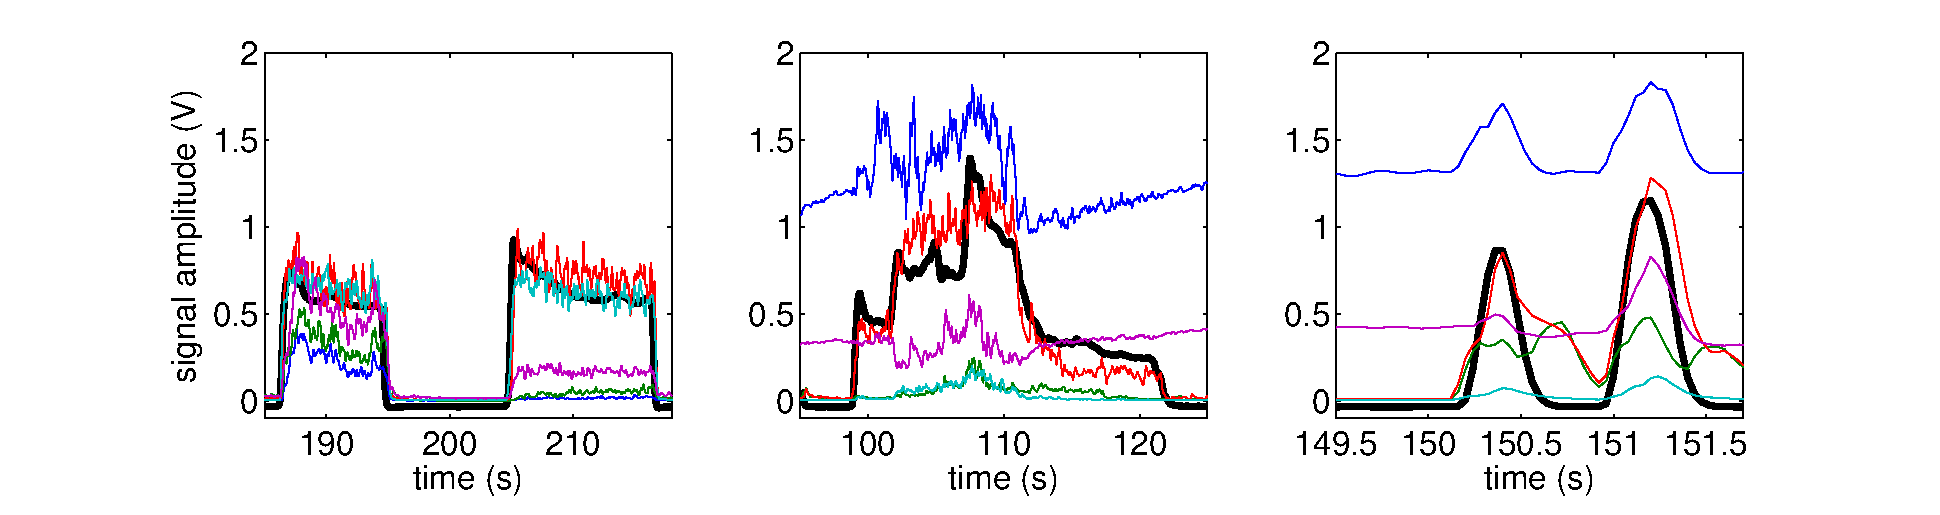
\includegraphics[width=\textwidth]{figs/figExamples}
  \caption{three examples of force (black thick line) and EMG
    signals (coloured thin lines). (left panel) Subject $1$ in the teacher imitation
    modality switches from \po\ to \pw\ at about $200$ seconds of activity --- notice
    the sharp change in relative average magnitude of the EMG signals, before and after
    the switch. (center and right panels) Subject $3$ in the mirror-box modality, slow
    and fast power grasping.}
  \label{fig:examples}
\end{figure*}

\subsection{Data pre-processing and preliminary analysis}

Both force and EMG signals were digitally filtered
to remove high-frequency noise components (II order low-pass FIR filter
with cut-off frequency at $5$Hz). After filtering, spectral analysis
reveals that the relevant bandwidth of the
EMG signal, as recovered form the elctrodes, and of the force signal,
lies below $10$-$12$Hz, so both signals were subsampled at $25$Hz.

Principal Component Analysis (PCA) was applied to the $5$ EMG signals in
each cycle, revealing that they can be linearly reduced to two losing,
on average, only $7.7\% \pm 4.4\%$ of the signal variance. Although this
loss would probably hinder classification and regression, and therefore
the $5$-dimensional original signals were used later on, this reduction
enables us to visualise the samples, tagging them according to the labels
(and therefore according to the grasp), and to qualitatively check
how well the subjects can produce different EMG
patterns when they are asked to perform different grasping
actions. Figure \ref{fig:PCA} shows the results, according to each
subject and modality.

\begin{figure*}[!ht] \centering
  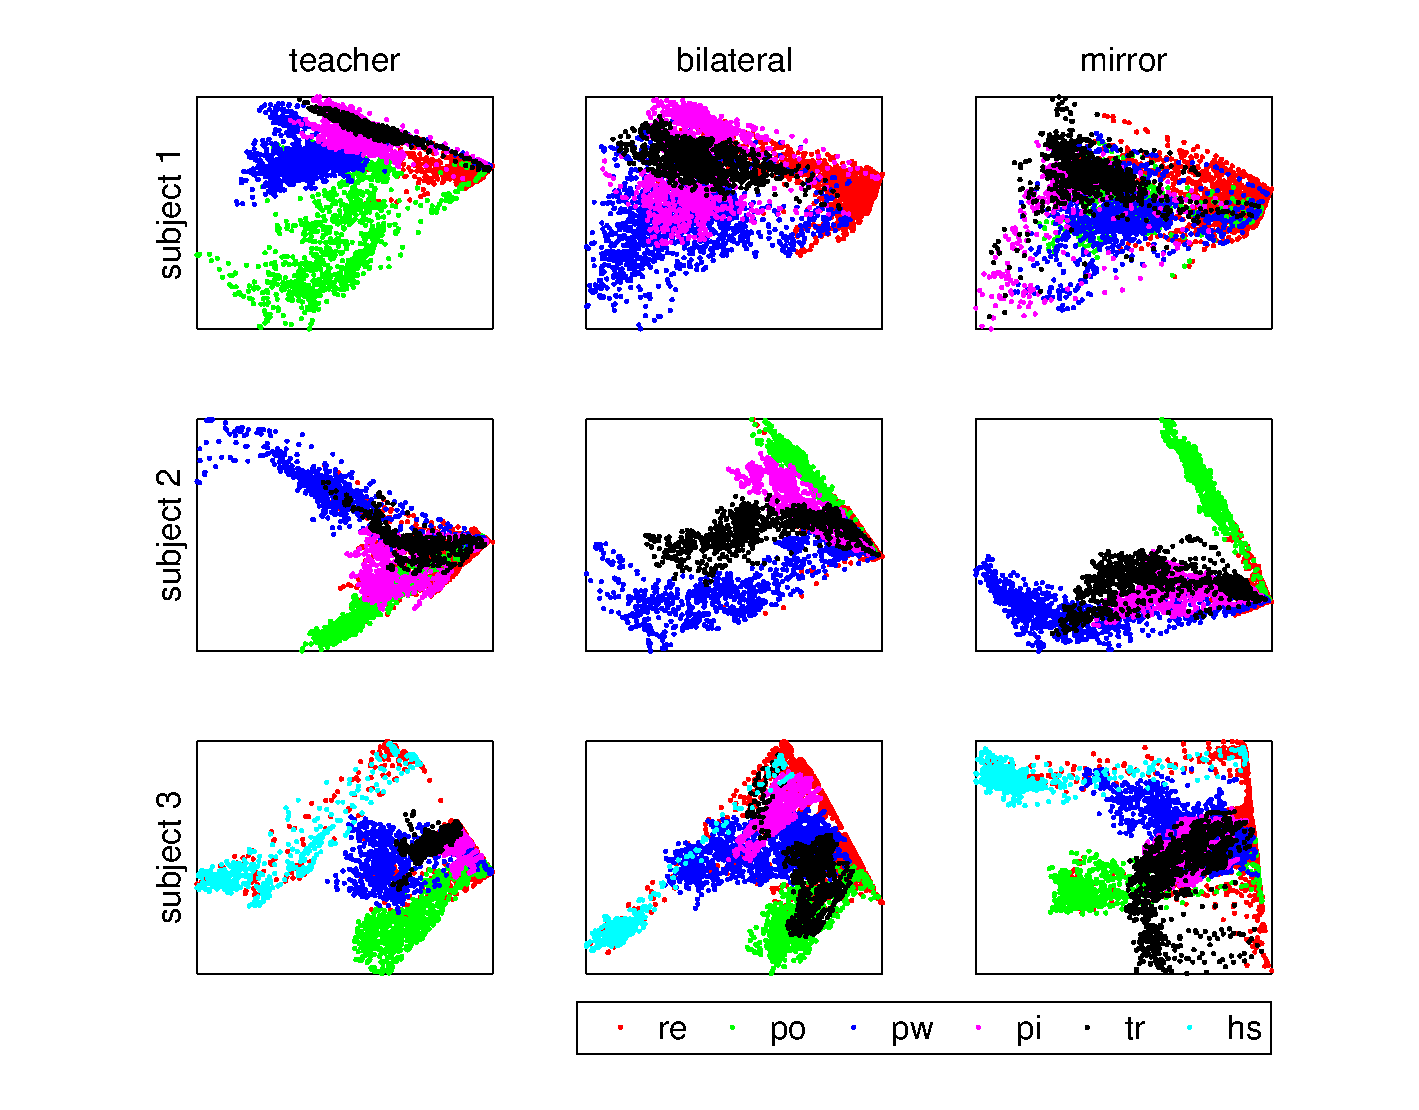
\includegraphics[width=\textwidth]{figs/figPCA}
  \caption{visualisation of the PCA-reduced EMG signals.}
  \label{fig:PCA}
\end{figure*}

As is apparent from the Figure, all subjects can produce distinct signals
according to the required type of grasp. In particular,
notice how two very similar grasp types, i.e.,
\pi\ and \tr, are qualitatively discernible on almost each graph.
Notice that PCA being so effective in reducing the
dimensionality of the EMG signals two does not imply that
two electrodes would suffice to obtain the same results. In fact, PCA coefficients
consistently show the same magnitude, meaning that each electrode
is required.

\subsection{Classification / regression method}
\label{subsec:method}

The good performance of Support Vector Machines (SVMs) applied to similar
problems is known since \cite{smagt06}. SVMs are
statistical learning machines \cite{v-edbed-82} which build an approximated map between
samples drawn from an input space (under the standard i.i.d. sampling hypothesis)
and a set of labels (classification) or a real value (regression).
The map is a weighted sum of basic functions chosen a priori
via the so-called kernel (hence the term \emph{kernel methods}), each of
which is centered on a sample.
The weights are found by minimising a cost functional which is the sum of
a loss function, punishing the error on the samples, and a regulariser, punishing
over-complex solutions. For a comprehensive tutorial on SVMs please refer to
\cite{Burges98,SmolaTut2004}.

Maps found by SVMs are sparse, meaning that some (practically, most) of the
weights found by minimisation are zero.
Those samples for which the weight is not zero, that is, those which actually
contribute to the map, are called \emph{Support Vectors}
(SVs), and their number is usually much smaller
than the total number of samples used in the training phase --- this is why
prediction with SVMs is in practice rather fast \cite{Cristianini00}. The
ratio between the number of SVs and the number of samples is then a good index
to measure how difficult a problem is: the smaller the ratio, the easier
the problem, indicating that a few samples are sufficient to
fully determine the map. In classification, this means that samples with different
labels are well separated in the input space; in regression, it means that a
simple relationship exists between the samples and the target values.
The sparsity of SVM models is extremely useful in our context, since
smaller models also mean higher chance of miniaturising them and using them
in pratice on a prosthesis.

In our case, the input space is $\RR^5$, one coordinate for each EMG
electrode; EMG signals are fed to the SVM as they are, sample by sample. The labels are
(a subset of) $\{\re,\po,\pw,\pi,\tr,\hs\}$ while the regression value is exactly the
force value as read from the force sensor. No feature extraction besides the low-pass
filtering is, therefore, employed on the signals.

As is standard, we use a Gaussian kernel both for classification and regression.
Multi-class classification is realised via the all-pairs schema,
in which a quadratic number of SVMs are trained to discriminate pairs of grasp
postures, and then a final decision is made according to a voting criterion.
Regression is done using the $\epsilon$-SVR technique, which neglects errors smaller
than a tolerance threshold $\epsilon>0$, here set at the default value of $0.1$.
Multi-class classification and $\epsilon$-SVR are
provided by \emph{libsvm} v2.83 \cite{ChangL01} in the Matlab wrapped version.

For classification, the performance index is the \emph{weighted accuracy},
that is the average of the percentages of correctly predicted labels of type
$i$, divided by the number of labels $i$ in the testing set:

$$ \sum_{i \in \{\re,\po,\pw,\pi,\tr,\hs\}}	\frac{c_i}{n_i} $$

\noindent where $n_i$ is the number of samples tagged with the label $i$
in the testing set and $c_i$ is the number of correctly predicted labels of type $i$.
This measure, as opposed to the more standard overall ratio of correctly
predicted labels and number of samples, has the advantage of adjusting the
importance of each label according to how often it appears in the
testing set. For example, in general there are more \re\ labels than others,
since the resting condition appears both at the beginning
of the experiment and in-between the grasps, therefore this label must be
weighted \emph{less} than the others, since it is more easily found in the testing
set. For regression, the performance index is the root mean-square error (RMSE),
normalised over the range of the force signal. This values characterises
the error in regression as a percentage of the maximum amplitude of the target
signal.

In both cases, in order to avoid the ominous danger of overfitting the data,
two hyperparameters have to be found, $\gamma$ and $C$,
which account in turn for the width of the Gaussians used to build the
approximated solution and the weight assigned to the regulariser during minimisation of
the cost functional.
We find optimal values for $C$ and $\gamma$, as is standard, by logarithmic grid search:
for each pair $(C,\gamma)$ for $C=10^{1,\ldots,3}$ and $\gamma=\frac{10^{0,\ldots,2}}{5}$,
the generalisation error of a machine trained using that pair is estimated
via $5$-fold cross-validation; at the end the pair resulting in the best performance is
chosen as optimal. Training samples are normalised by subtracting the mean values
dimension-wise and dividing by the standard deviations; testing samples are normalised
using the mean and standard deviation of the training set.

After the optimal parameters are found, the generalisation error of the optimal machine
is evaluated via an \emph{outer} $10$-fold cross-validation,
in which for each fold the optimal parameters found during the previous step
are used to train an optimal machine on the training set of the split; the optimal
machine so obtained is then tested on the testing set left of the split.
This method, called \emph{nested cross-validation},
is deemed to be among the best ways to get an unbiased estimate of the generalisation
error of a machine learning method, since $(a)$ it de-couples the estimation of the
optimal parameters from that of the generalisation error, and $(b)$ it never tests
a machine on data which have been used for training, avoiding the so-called
resubstitution bias \cite{nestedCV}.
